\vspace{-2pt}
\subsection{Normalizing Across Vastly Different Apps}
\label{subsec:relativeEff}

Platform evaluation is key to UPA. Evaluating many applications poses two challenges: (a) normalizing performance metric for vastly different applications, and (b) fair aggregation of performances across all applications. This section introduces relative efficiency as a measure of performance across applications. \secref{subsec:aggregation} discusses the aggregation.

Platform design can optimize various goals, e.g., minimize energy consumption or maximize throughput, under various constraints (e.g., cost, area). In this work, we focus on maximizing energy efficiency, which combines performance and energy as a goal, with area (in number of ACCs) as a constraint. Eq.~\eqref{eq:pipe} calculates the energy efficiency ($EFF$) of the platform using the analytic model from \secref{subsec:ana}. In streaming, energy efficiency can be expressed as throughput [bytes/second] per watt of power~\cite{zhou2013energy}. Throughput is equal to output volume per iteration $D_{out}$ over the latency time $L$. The power is equal to energy consumption $EC$ over its latency $L$. \newtext{In the rest of this paper, the "efficiency" means "energy efficiency" ($EFF$) when the application(s) executed on the platform.}

\vspace{-8pt}
\begin{equation}
	EFF = \left. \frac{Th}{Power} \right\vert\ Th = \frac{D_{out}}{L},\ Power = \frac{EC}{L}
\label{eq:pipe}
\end{equation}

\newtext{
However, energy efficiency differs vastly across applications even with similar acceleration supporting. E.g., the applications with a large volume of output data have much better efficiency than other applications due to high throughput. 
Moreover, applications have differing potentials for efficiency. The computing-dense applications have a larger potential to increase their efficiency than the applications with less computing.
Hence, direct comparison or aggregation is not suitable. To fairly judge platform efficiency across applications, it needs to be normalized to some measure of an application's base efficiency or potential for efficiency increasing.
}

We consider two bounds for normalization. Pure software execution (SW) marks the lower bound. The upper bound is execution on an Own Optimal Dedicated Platform (ODP), which is individual to the particular application ignoring all others in the set. Given a ACC budget, each application has its own optimal platform, obtained through one application exploration, e.g. exhaustive search. As a result, an ODP is the efficiency upper boundary for its application but is not designed for other applications.

\newtext{
Using the two normalizations, Eq.~\eqref{eq:rel} defines two relative efficiencies balancing across applications. $rEFF_{SW}$ represents the  Efficiency Improvement of an application $a_i$ on platform $p_X$ over $SW$, and $rEFF_{ODP}$ represents the Efficiency Achievement of $a_i$ on $p_X$ relative to $ODP$.
In another view of efficiency achievement, $1 - rEFF_{ODP}$ represents how much the efficiency loss is from fully satisfied efficiency potential with the same  ACC budget.
}


\vspace{-8pt}
\begin{equation}
\begin{split}
	rEFF_{SW}(a_{i}, p_{X}) &= EFF(a_{i}, p_{X}) / EFF(a_{i}, p_{SW}) \\
	rEFF_{ODP}(a_{i}, p_{X}) &= EFF(a_{i}, p_{X}) / EFF(a_{i}, p_{ODP})
\label{eq:rel}
\end{split}
\end{equation}

For illustration, \figref{fig:eff} plots the relative efficiency of 40 OpenVX applications on one Unified Platform (UP, blue) with 10 ACCs. While the normalizations help reduce variations in efficiency, they don't eliminate all of the variation due to applications' potentials for efficiency. This poses a challenge for aggregation to evaluate a platform, since it should not over-represent high-efficiency applications.

\vspace{-4pt}
\begin{figure}[h]
	\centering
		\subfloat[Efficiency Improvement]{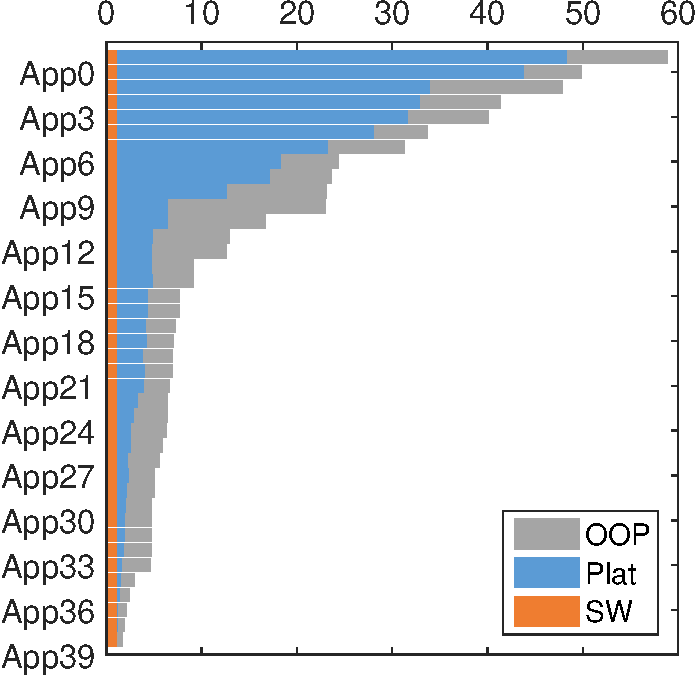
\includegraphics[width=.46\linewidth]{fig/effSW.pdf}\label{fig:effSW}}
		\hfill
		\subfloat[Efficiency Achievement]{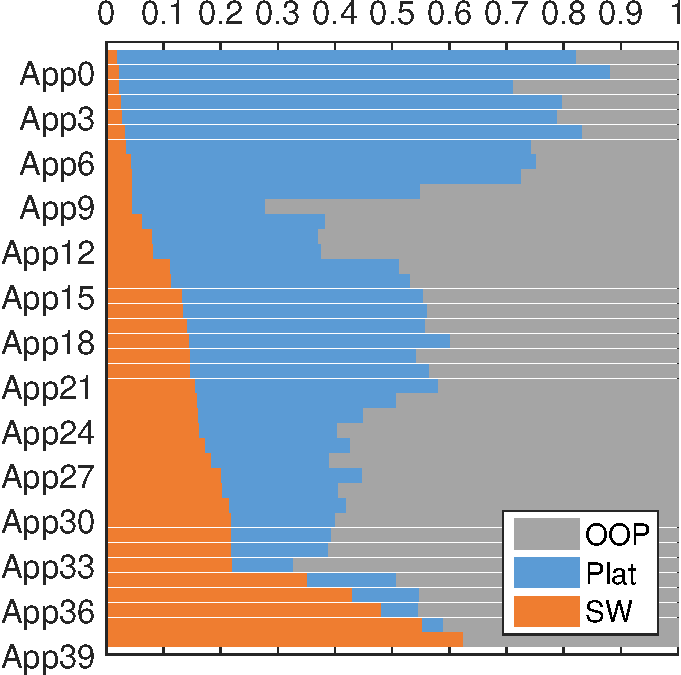
\includegraphics[width=.45\linewidth]{fig/effOOP.pdf}\label{fig:effOOP}}
    \vspace{-8pt}
	\caption{Relative Efficiency}
	\label{fig:eff}
    \vspace{-4pt}
\end{figure}